\documentclass{article}
\usepackage[utf8]{inputenc}
\usepackage[margin=1.0in]{geometry}
\usepackage{amsmath}
\usepackage{amssymb}
\usepackage{fancyhdr}
\usepackage{physics}
\usepackage{wrapfig}
\usepackage{hyperref}
\usepackage{multirow}
\usepackage{amsthm}
\usepackage{pgfplots}

\pgfplotsset{compat=1.16}



\renewcommand{\thesubsection}{\thesection\Alph{subsection}}
\renewcommand\qedsymbol{\square}



\title{Particle Physics PS1}
\author{Joe Crowley}
\date{October 2020}

\pagestyle{fancy}
\renewcommand{\headrulewidth}{0pt}
\renewcommand{\footrulewidth}{1pt}

\fancyhf{}
\rhead{
Joe Crowley \\
Physics 225 \\
Problem Set 2\\
}
\rfoot{Page \thepage}

\begin{document}  


\section{Questions on natural units}

\subsection{}
\textit{The cross section for the process $e^{+} e^{-} \rightarrow \mu^{+} \mu^{-}$ (via a virtual photon) is given by $\sigma=\frac{4 \pi}{3} \frac{\alpha^{2}}{E_{\mathrm{cm}}^{2}}$ in n.u., where $E_{\mathrm{cm}}$ is the total energy in the center-of-momentum frame. (This formula applies for $\left.E_{\mathrm{CM}}>>m_{\mu} .\right)$ What are the required dimensions of a cross section? Use this fact to restore any needed powers of $\hbar$ and $c$ to the cross section formula. Next, compute the numerical value of this cross section at $E_{\mathrm{CM}}=1 \mathrm{GeV}$ in the units of barns, where 1 barn $=1 \mathrm{b}=10^{-24} \mathrm{cm}^{2}$}

\begin{align*}
    [\sigma]&=[L]^{2}\\
    [L]^2 &= [E]^{-2}[E L ]^2\\
    \implies \sigma &= \frac{4 \pi}{3} \frac{\alpha^{2}}{E_{\mathrm{cm}}^{2}} (\hbar c)^2\\
    &= 8.68545 \times 10^{-36} \, \mathrm{m}^{2}\\
    &= 8.68545 \times 10^{-8} \,\mathrm{barns}
\end{align*}


\subsection{}
\textit{When a low energy photon scatters from an atomic electron, there is an energy regime in which $E_{B}<<E(\gamma)<<m_{e} .$ (Here $E_{B}$ is the atomic binding energy.) This is called Thomson scattering, and the cross section is given by
$$
\sigma\left(\gamma e^{-} \rightarrow \gamma e^{-}\right)=\frac{8 \pi}{3}\left(\frac{\alpha}{m_{e}}\right)^{2}
$$
Restore any needed powers of $\hbar$ and $c,$ and then evaluate the scattering cross section in $\mathrm{cm}^{2} .$ Hint: $\sigma=6.6 \times 10^{-25} \mathrm{cm}^{2}$}

\begin{align*}
    [\sigma]&=[L]^{2}\\
    [L]^2 &= [E]^{-2}[E L ]^2\\
    \implies \sigma\left(\gamma e^{-} \rightarrow \gamma e^{-}\right)&=\frac{8 \pi}{3}\left(\frac{\alpha}{m_{e} c^2 }\right)^{2}  (\hbar c)^2\\
    &= \frac{8 \pi}{3}\left(\frac{\alpha \hbar}{m_{e} c}\right)^{2}\\
    &=6.6 \times 10^{-29} \mathrm{m}^{2}\\
    &=6.6 \times 10^{-25} \mathrm{cm}^{2}
\end{align*}

\subsection{}
\textit{Bohr radius, Compton wavelength, and "classical" electron radius. Recall that, in n.u., the Bohr radius of the H-atom is $a_{0}=1 /\left(m_{e} \alpha\right)$ and the Compton wavelength of the electron is $\lambda_{C}=1 / m_{e} .$ From the discussion of Thomson scattering, you can see that we can define a length scale $r_{0}=$ $\alpha / m_{e}$ in which $\alpha$ is in the numerator. This quantity is called the classical electron radius. Make a table listing the values of these three quantities. We will later see that the Compton wavelength is extremely important, because it sets a length scale below which quantum field theory must be used rather than a single particle wave equation (for the given type of particle}

\begin{table}[]
    \centering
    \begin{tabular}{||c|c|c||}
        \hline\hline
         &  &\\
        $a_{0}$ & $\lambda_{c}$ & $r_{0}$ \\
         & & \\
        \hline & & \\$\frac{1}{\alpha m_{e}}$ & $\frac{1}{m_{e}}$ & $\frac{\alpha}{m_{e}}$ \\
         & & \\
        \hline & & \\ $0.529 \AA$ & $386 \mathrm{fm}$ & $2.82 \mathrm{fm}$ \\
         & & \\
        \hline\hline
    \end{tabular}
    \caption{Bohr radius, Compton wavelength, and "classical" electron radius.}
    \label{tab:my_label}
\end{table}




\newpage


\section{Simple relativity: Lorentz invariant quantities}
\textit{Consider two arbitrary four vectors, $a=\left(a^{0}, \vec{a}\right)$ and $b=\left(b^{0}, \vec{b}\right)$.}

\subsection{}
\textit{Show explicitly that the dot product
$$
a \cdot b=a^{0} b^{0}-\vec{a} \cdot \vec{b}
$$
is invariant under a Lorentz transformation along the $z$ axis. In other words show that $a^{\prime} \cdot b^{\prime}=a \cdot b,$ where $a^{\prime}$ and $b^{\prime}$ are the Lorentz-transformed four vectors.}
\begin{align*}
    a \cdot b&=a^{\prime} \cdot b^{\prime}\\
    (a^\prime)^{\mu} (b^\prime)_{\mu}&=\Lambda_{\;\rho}^{\mu} a^{\rho} \Lambda_{\mu}^{\;\sigma} b_{\sigma}\\
    &=\Lambda^{\mu} _{\;\rho} \Lambda_{\mu}^{\;\sigma} a^{\rho} b_{\sigma}\\
    &=\delta_{\rho}^{\sigma} a^{\rho} b_{\sigma} \\
    &= a^{\rho} b_{\rho} \\
    &= a \cdot b
\end{align*}

\begin{equation*}
    \boxed{ a \cdot b=a^{\prime} \cdot b^{\prime}}
\end{equation*}

\subsection{}
\textit{Suppose that two four-vectors are given by $a=(10.5,4.3,-5.6,7.9)$ (in some units) and $b=(-22.6,-3.5,6.6,50.4)$ (in some other units). Suppose that in another reference frame, $a^{\prime}=(7.777,4.3,-5.6,-3.556) .$ What are the parameters $\beta$ and $\beta \gamma$ for the Lorentz transformation? Compute $b^{\prime}$ and verify that $a \cdot a=a^{\prime} \cdot a^{\prime}$ and $a \cdot b=a^{\prime} \cdot b^{\prime}$}

The lorentz boost is along the z axis, because the x and y components of $a$ remain unchanged. Therefore, the equations for the primed variables are: 
\begin{align*}
t^{\prime}&=\gamma t-\beta \gamma z \\
z^{\prime}&=\gamma z-\beta \gamma t \\
\end{align*}

Solving these equations for $\gamma$ and $\beta\gamma$,

\begin{align*}
\gamma&=\frac{t t^{\prime}-z z^{\prime}}{t^{2}-z^{2}}=2.29412 \\
\beta \gamma&=\frac{z t^{\prime}-t z^{\prime}}{t^{2}-z^{2}}=2.06472
\end{align*}

Verifying the lorentz invariance of $a^2 = (a^\prime)^2$,

\begin{align*}
a \cdot &a=-2.01 \\
a^{\prime} \cdot a^{\prime}&=-2.013
\end{align*}

\begin{align*}
b \cdot b&=-2085.21 \\
b^{\prime} \cdot b^{\prime}&=-2085.07
\end{align*}


\subsection{}
\textit{Suppose a particle has four-momentum $p=(E, \mathbf{p})$ in some reference frame. What is the Lorentz transformation to the CM frame, where $\mathbf{p}^{\prime}=0 ?$ You may choose $\mathbf{p}$ to point in a particular direction for convenience. In the CM frame, what is the interpretation of $E ?$ Given this, what is the interpretation of $E^{2}-\mathbf{p}^{2}$ in an arbitrary reference frame?}

\begin{equation}
\left(\begin{array}{l}
m \\
0 \\
0 \\
0
\end{array}\right)=\left(\begin{array}{llll}
\gamma & 0 & 0 & -\beta \gamma \\
0 & 1 & 0 & 0 \\
0 & 0 & 1 & 0 \\
-\beta \gamma & 0 & 0 & \gamma
\end{array}\right)\left(\begin{array}{l}
E \\
0 \\
0 \\
p
\end{array}\right)
\end{equation}

\begin{align*}
\beta \gamma&=\frac{m p}{E^{2}-p^{2}} \\
\gamma&=\frac{E m}{E^{2}-p^{2}}
\end{align*}

in an abitrary reference frame, $m^{2}=E^{2}-\mathbf{p}\;^{2}$ is the lorentz invariant  mass squared.

\subsection{}
\textit{A particle has four-momentum $p=(4.0,0.0,0.0,2.5315) \mathrm{GeV} .$ What is the mass of a particle? What particle is this?}

\begin{align*}
    m&=\sqrt{p^{\mu} p_{\mu}}\\
    &=\sqrt{9.59151 \mathrm{GeV}^{2}}\\
    &=3.097 \text { GeV }
\end{align*}

this is the $J/\Psi$ meson, with mass 3.0969 GeV.

\newpage


\section{Decay of a free photon?}
\textit{Using relativity, show that the process $\gamma \rightarrow e^{+} e^{-}$ cannot occur in the vacuum. Here the photon is a free particle, not a virtual photon. Your argument should be mathematical, not just verbal.}

In the center of momentum frame
$$
\mathbf{p}_{\text {tot }}=\mathbf{p}_{\gamma}=\vec{p_1}+\vec{p_2}=0
$$
but that implies
$$
\mathbf{p}_{\gamma}=0
$$
and the energy of the photon $E_{\gamma} = \left|\mathbf{p}_\gamma\right|$ imply that in the CM frame of the photon it has $E_\gamma = 0$.



\newpage


\section{}
\textit{Let $G$ be a group. Prove that}

\subsection{}
\textit{The identity element of $G$ is unique.}

\begin{proof}
From the group axioms,
$$
\exists e \in G \; \text {such that} \forall a \in G \quad e \cdot a=a \cdot e=a
$$
Suppose $\exists f \in G \; \text {such that} \forall a \in G \quad f \cdot a=a \cdot f=a$. Let $a = e$ and determine 
\begin{align*}
    f \cdot e  &= e \cdot f  \\
    f  &=  e \cdot f \\
    f &=e
\end{align*}
$\therefore$ The identity $e$ is unique.
\end{proof}


\subsection{}
\textit{Every element $a \in G$ has a unique inverse in $G$.}

\begin{proof}
Suppose $\forall a \in G \; \exists (b,c) \in G \; \text {such that} $
$$
a \cdot b=b \cdot a=a \cdot c=c \cdot a=e
$$
This implies 
\begin{align*}
a \cdot b &= a \cdot c \\
(b \cdot a) \cdot b &= (b\cdot a) \cdot c \\
e \cdot b &= e \cdot c \\
b &= c
\end{align*}
$\therefore$ the inverse $b$ is unique.
\end{proof}

\newpage


\section{Kinematics of scattering in a fixed-target experiment.}
\textit{A beam of particles with mass $M_{A}$ and energy $E_{A}$ is incident on a target containing particles of mass $M_{B}$ at rest, resulting in the process $A+B \rightarrow$ $1+2+\ldots+N .$ The final-state particles have masses $m_{1}, m_{2}, \ldots, m_{N}$}

\begin{figure}[h!]
    \centering
    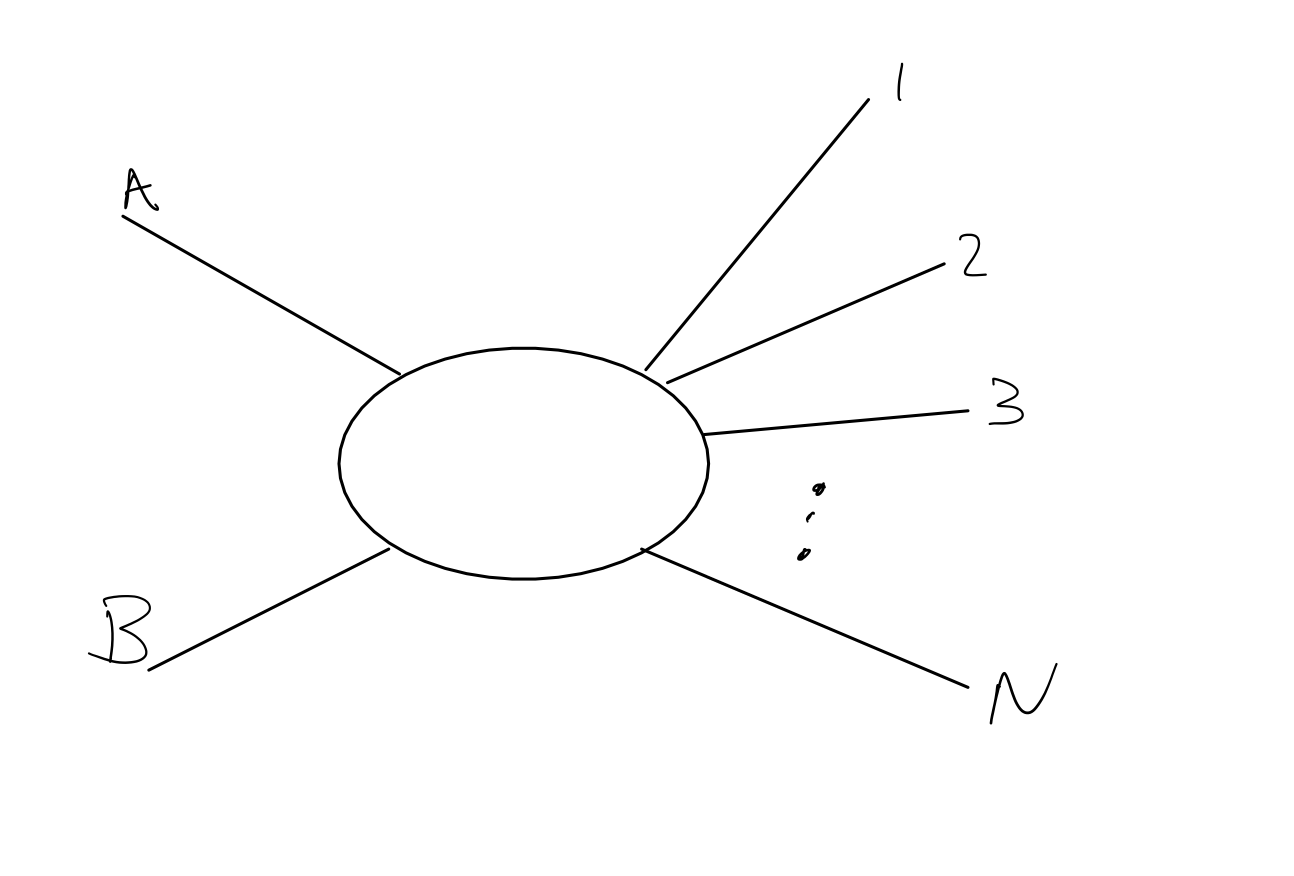
\includegraphics[width=0.4\textwidth]{figures/problem_5.png}
    \label{fig:my_label}
\end{figure}
\subsection{}
\textit{True or false: $M_{A}+M_{B}=m_{1}+m_{2}+\ldots+m_{N} .$ If true, explain why. If not, give an alternative statement.}


False. Conservation of four-momentum:  
$$
p^\mu_{A}+p^\mu_{B}=p^\mu_{1}+p^\mu_{2}+\ldots+p^\mu_{N}.
$$
\subsection{}
\textit{Compute the minimum value of the energy of particle $\mathrm{A}, E=E_{A}^{\min },$ for the process to be kinematically allowed.}

\begin{align*}
    \left(p_{A}+p_{B}\right)^{2}&=\left(\sum_{f=1}^{N} p_{f}\right)^{2}\\
    p_{A}^{2}+p_{B}^{2}+2 p_{A} \cdot p_{B}&=\left(\sum_{f=1}^{N} p_{f}\right)^{2}\\
    m_{A}^{2}+m_{B}^{2}+2 E_{A} m_{B}&=\left(\sum_{f=1}^{N} p_{f}\right)^{2}\\
\end{align*}

\begin{equation*}
\boxed{
    E_{A}=\frac{\left(\sum_{f=1}^{N} p_{f}\right)^{2}-m_{A}^{2}-m_{B}^{2}}{2 m_{B}}
    }
\end{equation*}


\subsection{}
\textit{Consider the case of a $\tau$ neutrino with energy $E_{\nu}$ that is incident on a neutron at rest. What is the minimum value of $E_{\nu}^{\min }$ for the neutrino to produce a $\tau$ -lepton via the process $\nu_{\tau}+n \rightarrow \tau^{-}+p ?$ (You may neglect the neutrino mass in the calculation. You may use $m_{p}=938 \mathrm{MeV}, m_{n}=940$ $\mathrm{MeV},$ and $\left.m_{\tau}=1777 \mathrm{MeV} .\right)$}

$$
E_{\nu_{\tau}}=\frac{\left(938\, \mathrm{MeV}+1777 \,\mathrm{MeV}\right)^{2}-940 \,\mathrm{MeV}^{2}}{2(940\, \mathrm{MeV})} = 3.45  \,\mathrm{GeV}
$$


\newpage


\section{Colliding electron and positron beams at asymmetric energies.}
\textit{In the PEP-II storage ring at SLAC, the electron and positron beam energies were, respectively, $E_{1}=9.0 \mathrm{GeV}$ and $E_{2}=3.1 \mathrm{GeV} .$ The beams collided head on.}
\subsection{}
\textit{What is the total energy of the $e^{+} e^{-}$ system in the CM frame (the frame in which the total momentum is zero)?}

\begin{align*}
    E_{CM}^{2}&=\left(p_{1}+p_{2}\right)^{2}\\
    &= E_{tot}^{2} - \mathbf{p}_{tot}^2\\
    &\approx  (E_- + E_+)_{tot}^{2} - (E_- - E_+)_{tot}^2\\
    &=  (9\, \mathrm{GeV} + 3.1\, \mathrm{GeV})^{2} - (9\, \mathrm{GeV} - 3.1\, \mathrm{GeV})^2\\
    &= 10.56 \, \mathrm{GeV} \\
\end{align*}


\subsection{}
\textit{What $\Upsilon$ (a $b \bar{b}$ system) state is closest to this energy? These mesons are created in very large quantities (hundreds of millions) at PEP-II. What is the dominant decay mode of this $\Upsilon$ state?}

The mass of the $\Upsilon(4S) \sim E_{CM}$. The main decay modes of the $\Upsilon(4S)$ are tabulated below. 

\begin{table}[h!]
    \centering
    \begin{tabular}{||c|c||}
        \hline \hline & \\
        Mode & $\frac{\Gamma_i}{\Gamma}$  \\& \\
         \hline & \\
         $B\bar B$ & $> 96\%$  \\
         \hline & \\
         $B^+ B^-$& $(51.4 \pm 0.6)\%$ \\
         \hline & \\
         $B^0 \bar{B}^0$& $(48.6 \pm 0.6)\%$ \\
         \hline\hline
    \end{tabular}
    \caption{Decay modes of the $\Upsilon(4S)$}
    \label{tab:my_label}
\end{table}

\subsection{}
\textit{What are the velocity $\beta$ and the factor $\beta \gamma$ for the Lorentz transformation from the lab frame to the CM frame?}

\begin{equation*}
    \left(E_{\mathrm{CM}}, 0,0,0\right)=\left(\begin{array}{cccc}
\gamma & 0 & 0 & -\beta \gamma \\
0 & 1 & 0 & 0 \\
0 & 0 & 1 & 0 \\
-\beta \gamma & 0 & 0 & \gamma
\end{array}\right)\left(\begin{array}{c}
E_{1}+E_{2} \\
\mathbf{p}_{1}+\mathbf{p}_{2}
\end{array}\right)
\end{equation*}

\begin{align*}
    \gamma&=\frac{\left(E_{1}+E_{2}\right) E_{\mathrm{CM}}}{E_{1}^{2}+E_{2}^{2}+2 E_{1} E_{2}-p_{1}^{2}-p_{2}^{2}-2 p_{1} p_{2}}\\
    \beta \gamma&=\frac{\left(p_{1}+p_{2}\right) E_{c m}}{p_{1}^{2}+p_{2}^{2}+2 p_{1} p_{2}-E_{1}^{2}-E_{2}^{2}-2 E_{1} E_{2}}
\end{align*}

Plugging in values gives 
\begin{align*}
\gamma&=9.32848 \times 10^{7} \\
\beta \gamma& =9.32848 \times 10^{7}
\end{align*}

\subsection{}
\textit{What are the beam energies in the CM frame?}

\begin{equation*}
    E_{1}=\frac{E_{\mathrm{C M}}^{2}+m_{1}^{2}-m_{2}^{2}}{2 E_{m}}
\end{equation*}

\begin{equation*}
    E_{2}=\frac{E_{\mathrm{C M}}^{2}+m_{2}^{2}-m_{1}^{2}}{2 E_{m}}
\end{equation*}

$$
E_{1}=E_{2}=\frac{E_{\mathrm{CM}}}{2} =5.28 \, \mathrm{Gev}
$$

\subsection{}
\textit{Using the web, try to find a description or a photo of the inside of the PEP-II ring. How were the two beams stored in this accelerator? What did it look like inside the tunnel?}

Two beam pipes were stacked atop each other with the high energy ring being an uprade from PEP, the low energy ring was newly constructed.
\begin{figure}[h!]
\centering
    \begin{minipage}{.5\textwidth}
        \centering
        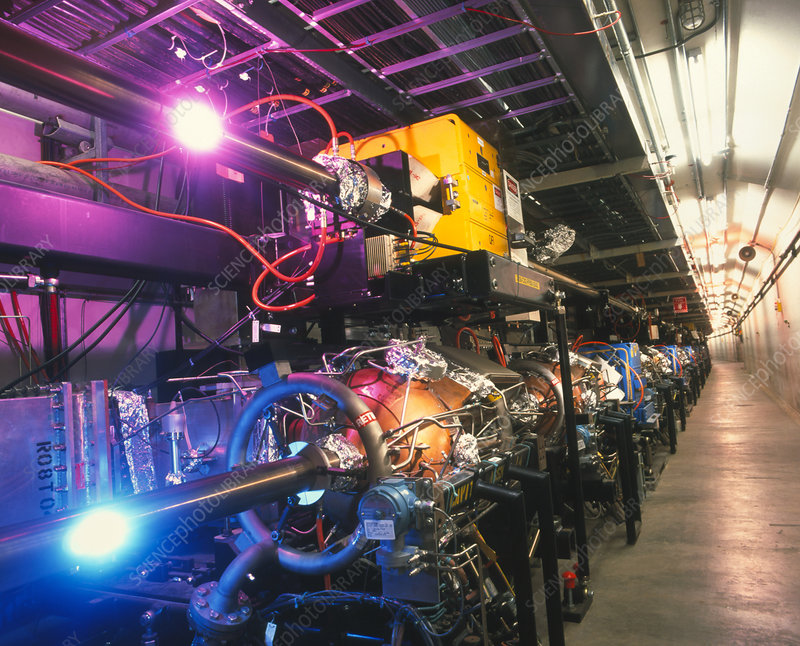
\includegraphics[width=0.5\linewidth]{figures/storage_rings.jpg}
        \caption{Storage rings for PEP-II}
        \label{fig:my_label}
    \end{minipage}
    \begin{minipage}{.5\textwidth}
        \centering
        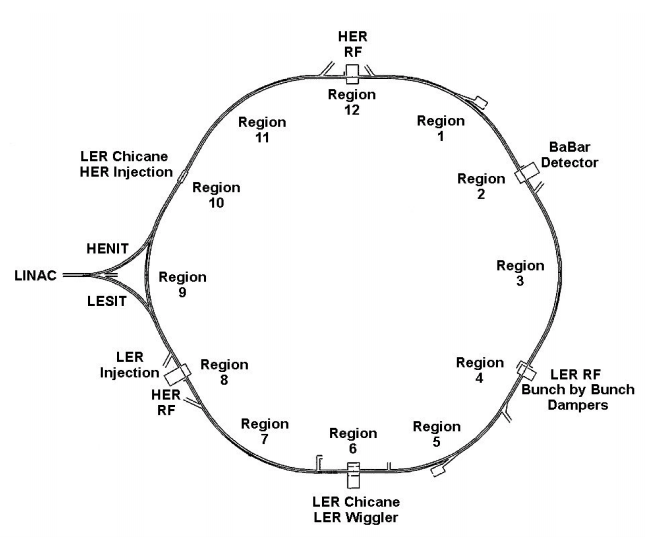
\includegraphics[width=0.5\linewidth]{figures/pepII rings.png}
        \caption{Schematic representation of PEP-II}
        \label{fig:my_label}
    \end{minipage}
\end{figure}

\newpage


\section{Momenta in two body decay of a particle. }
\textit{In Lecture $4,$ we calculated the energies of the outgoing particles 1 and 2 in the decay $A \rightarrow 1+2 .$ For the record let's calculate the magnitudes of the corresponding momenta. Show that
$$
\left|\mathbf{p}_{1}\right|=\left|\mathbf{p}_{2}\right|=\frac{\lambda^{1 / 2}\left(m_{A}^{2}, m_{1}^{2}, m_{2}^{2}\right)}{2 m_{a}}
$$
where the function $\lambda$ is given by
$$
\lambda(x, y, z)=x^{2}+y^{2}+z^{2}-2 x y-2 x z-2 y z
$$}


Conservation of four-momentum states that
\begin{align*}
p_{A} &=p_{1}+p_{2} \\
p_{2}^{2} &=\left(p_{A}-p_{1}\right)^{2} \\
p_{2}^{2}&=p_{A}^{2}+p_{1}^{2}-2 p_{A} p_{1}\\
m_{2}^{2}&=m_{A}^{2}+m_{1}^{2}-2 m_{A} E_{1} \\
\end{align*}

Solving for $E_1$,

\begin{equation*}
E_{1}=\frac{m_{A}^{2}-m_{2}^{2}+m_{1}^{2}}{2 m_{A}}
\end{equation*}

Using the Lorentz invariant mass squared,
\begin{align*}
    \left|\mathbf{p}_{1}\right|&=\sqrt{E_{1}^{2}-m_{1}^{2}}\\
    &=\sqrt{\left(\frac{m_{A}^{2}-m_{2}^{2}+m_{1}^{2}}{2 m_{A}}\right)^{2}-m_{1}^{2}}\\
    &= \sqrt{\frac{1}{2} m_{1}^{2}-\frac{1}{2} m_{2}^{2}+\frac{1}{4} \frac{m_{1}^{4}}{m_{A}^{2}}-\frac{1}{2} \frac{m_{1}^{2} m_{2}^{2}}{m_{A}^{2}}+\frac{1}{4} \frac{m_{2}^{4}}{m_{A}^{2}}+\frac{1}{4} m_{A}^{2}-m_{1}^{2}}\\
    &=\sqrt{\frac{m_{1}^{4}-2 m_{1}^{2} m_{2}^{2}+m_{2}^{4}-2 m_{1}^{2} m_{A}^{2}-2 m_{2}^{2} m_{A}^{2}+m_{A}^{4}}{4 m_{A}^{2}}}\\
\end{align*}
With $\lambda(x, y, z)=x^{2}+y^{2}+z^{2}-2 x y-2 x z-2 y z$, 
\begin{equation*}
    \left|\mathbf{p}_{1}\right|=\frac{\sqrt{\lambda\left(m_{A}^{2}, m_{1}^{2}, m_{2}^{2}\right)}}{2 m_{A}}
\end{equation*}

Since $\lambda(x, y, z) =\lambda(x, z, y)$,

$$
\boxed{
\left|\mathbf{p}_{1}\right|=\left|\mathbf{p}_{2}\right|=\frac{\lambda^{1 / 2}\left(m_{A}^{2}, m_{1}^{2}, m_{2}^{2}\right)}{2 m_{a}}}
$$

\newpage


\section{}
\textit{Mandelstam variables. Consider a scattering process $1+2 \rightarrow 3+4,$ where the 4 -momenta of the particles are $p_{1}, p_{2}, p_{3},$ and $p_{4} .$ The Mandelstam variables are the Lorentz-invariant quantities
$$
\begin{aligned}
s &=\left(p_{1}+p_{2}\right)^{2} \\
t &=\left(p_{3}-p_{1}\right)^{2} \\
u &=\left(p_{1}-p_{4}\right)^{2}
\end{aligned}
$$
These variables provide an alternate way to specify the same information that is contained in the (Lorentz-invariant) inner products of the four momenta.}
\subsection{}
\textit{Show that
$$
s+t+u=m_{1}^{2}+m_{2}^{2}+m_{3}^{2}+m_{4}^{2}
$$}

\begin{align*}
s+t+u &=\left(p_{1}+p_{2}\right)^{2} +\left(p_{3}-p_{1}\right)^{2}+\left(p_{1}-p_{4}\right)^{2}\\
&= p_{1}^{2}+p_{2}^{2}+p_{3}^{2}+p_{1}^{2}+p_{1}^{2}+p_{4}^{2} +2 p_{1} p_{2}-2 p_{3} p_{1}-2 p_{1} p_{4}\\
&=3 m_{1}^{2}+m_{2}^{2}+m_{3}^{2}+m_{4}^{2}+2 E_{1} E_{2}-2 \vec{p}_{1} \cdot \vec{p}_{2}-2\left(E_{3} E_{1}-\vec{p}_{3} \cdot \vec{p}_{1}\right)-2\left( E_{4} E_{1}-\vec{p}_{4} \cdot \vec{p}_{1}\right)\\
&= 3 m_{1}^{2}+m_{2}^{2}+m_{3}^{2}+m_{4}^{2} +2 E_{1}\left(E_{2}-E_{3}-E_{4}\right)+2 \vec{p}_{1}\, ^{2}\left(-\overrightarrow{p_{2}}+\overrightarrow{p_{3}}+\overrightarrow{p_{4}}\right)\\
&=3 m_{1}^{2}+m_{2}^{2}+m_{3}^{2}+m_{4}^{2}-2 p_{1}^{2}\\
&=3 m_{1}^{2}+m_{2}^{2}+m_{3}^{2}+m_{4}^{2}-2 m_{1}^{2} \\
&= m_{1}^{2}+m_{2}^{2}+m_{3}^{2}+m_{4}^{2}
\end{align*}

$$
\boxed{
s+t+u=m_{1}^{2}+m_{2}^{2}+m_{3}^{2}+m_{4}^{2}
}
$$

\newpage
\subsection{}
\textit{Compute $s, t,$ and $u$ in the CM frame in the relativistic limit $m_{i}=0$ Express the result in terms of the CM-frame scattering angle $\theta$ and the magnitude of the momentum of either particle in the CM frame, $\left|\mathbf{p}_{C M}\right|$. Compute $s+t+u$ for this case.}


\begin{align*}
\lim _{m_i \rightarrow 0} s=p_{1} p_{2}=p_{3} p_{4} \\
\lim _{m_i \rightarrow 0} t=-2 p_{1} p_{3}=-2 p_{2} p_{4} \\
\lim _{m_{i} \rightarrow 0} u=-2 p_{1} p_{4}=-2 p_{3} p_{2}
\end{align*}

\begin{align*}
p_{1}=(-E, 0,0, -E) \\
p_{2}=(-E, 0,0, E) \\
p_{3}=(E, E \sin \theta, 0, E \cos \theta) \\
p_{4}=\left(E,-E \sin \theta, 0,-E \cos \theta\right)
\end{align*}

\begin{align*}
    s&=(p_1+p_2)^2=(-2 E,0,0,0)^2=4 E^2\\
    t&=(p_1+\text{p3})^2=(E-E \cos (\theta )) (E \cos (\theta )-E)-E^2 \sin ^2(\theta )=2 E^2 (\cos (\theta )-1)\\
    u&=(p_1+\text{p3})^2=(E (-\cos (\theta ))-E) (E \cos (\theta )+E)-E^2 \sin ^2(\theta )=-2 E^2 (\cos (\theta )+1)\\
\end{align*}

\begin{equation*}
    s+t+u=-2 E^2 \sin ^2(\theta )+4 E^2+(E \cos (\theta )+E) (E (-\cos (\theta ))-E)+(E \cos (\theta )-E) (E-E \cos (\theta ))=0
\end{equation*}

\begin{equation*}
    \left|\vec{p}_{\mathrm{CM}}\right|=\frac{E_{\mathrm{CM}}}{2}
\end{equation*}

\newpage


\section{Charged pion decay.}
\textit{(Based on Griffiths problem 3.15 ) A pion traveling at speed $v$ in the lab frame decays into a muon and a neutrino, $\pi^{-} \rightarrow \mu^{-} \bar{\nu}_{\mu}$}
\subsection{}
\textit{What is the branching fraction for this decay?}
$$
\frac{\Gamma}{\Gamma_{to t}}=(99.98770 \pm 0.00004) \%
$$


\subsection{} 
\textit{What is the second most common $\pi^{-}$ decay?}

\begin{align*}
\pi^{-} &\rightarrow \mu{\bar{\nu}_{\mu}} \gamma\\
\frac{\Gamma}{\Gamma_{\text {tot }}}&=(2.00 \pm 0.25) \times 10^{-4}
\end{align*}


\subsection{} 
\textit{Neutrino beams are created by arranging for a beam of high-momentum charged pions to decay in a long beam pipe. What kind of neutrinos are mainly created in such beams?}

Overwhelmingly muon neutrinos

\subsection{} 
\textit{If the neutrino emerges at $90^{\circ}$ to the original pion direction, at what angle does the $\mu$ come off? Discuss the behavior of this result. Hint: $\tan \theta=$ $\left(1-m_{\mu}^{2} / m_{\pi}^{2}\right) /\left(2 \beta \gamma^{2}\right)$}


\begin{figure}[h!]
    \centering
    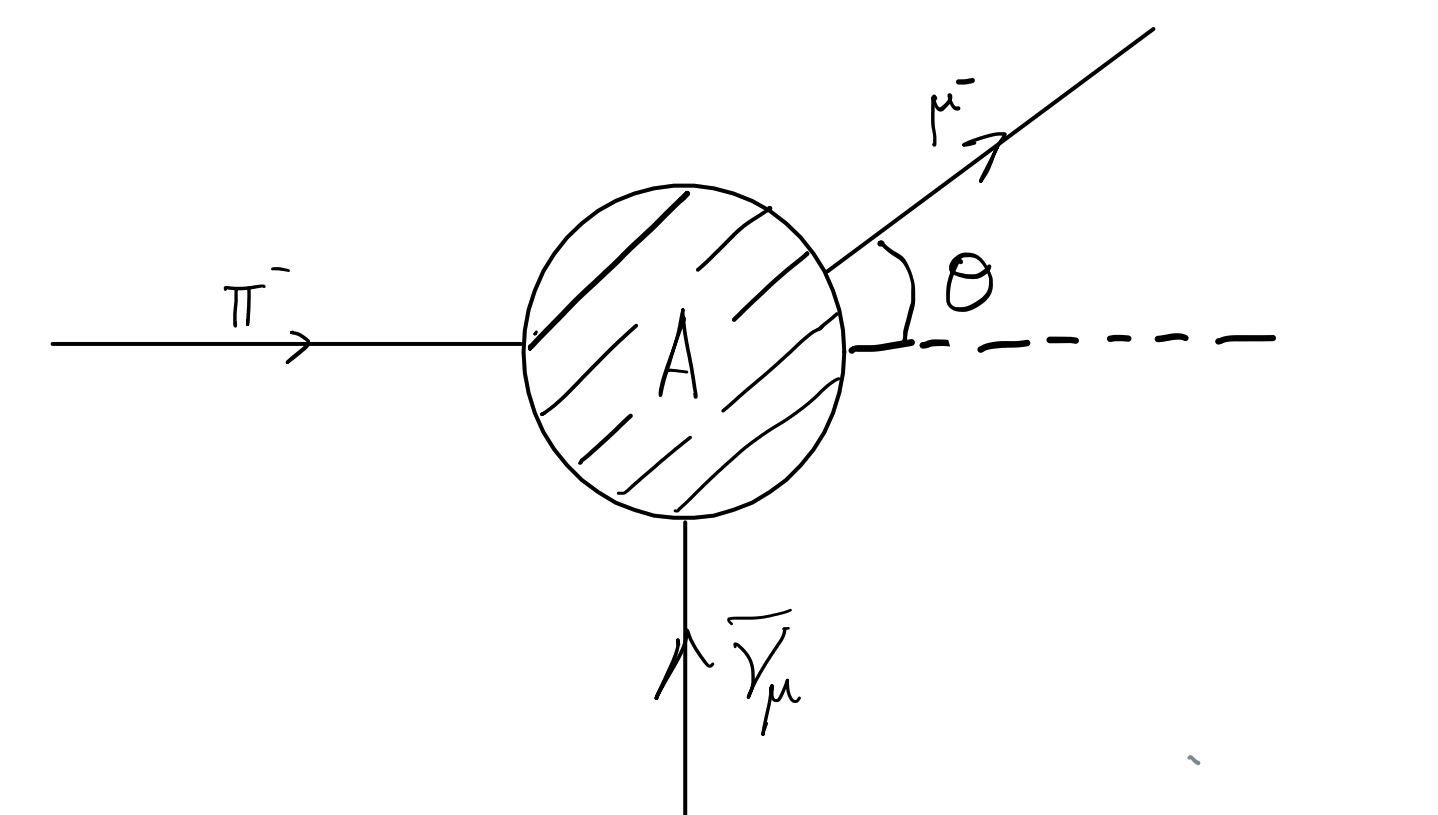
\includegraphics[width=0.5\textwidth]{figures/problem_9.png}
    \label{fig:my_label}
\end{figure}


\begin{align*}
    p_{\pi}&=p_{\mu}+p_{\nu_{\mu}}\\
    p_{\mu}^{2}&=\left(p_{\pi}-p_{\nu}\right)^{2}\\
    m_{\mu}^{2}&=m_{\pi}^{2}+m_{\nu}^{2}-2 p_{ \pi} p_{\nu}\\
    &= m_{\pi}^{2}+m_{\nu}^{2}-2 E_{\pi} E_{\nu} \\
\end{align*}

Assuming $m_{\nu} \approx 0$, $E_{\nu}=\left|\vec{p}_{\nu}\right|$, 

$$m_{\mu}^{2}=m_{\pi}^{2}-2 \gamma m_{\pi}\left|\vec{p}_{\nu}\right|$$
$$\left|p_{\nu}\right|=\frac{m_{\pi}^{2}-m_{\mu}^{2}}{2 \gamma m_{\pi}}$$

\begin{align*}
    \vec{p}_{\nu} \cdot \vec{p}_{\pi}&=0\\
    \implies \left|\vec{p}_{\mu}\right| \cos \theta&=\left|\vec{p}_{\pi}\right|\\
    \left|\vec{p}_{\mu}\right| \sin \theta&=\left|\vec{p}_{\nu}\right|\\
\end{align*}

\begin{align*}
    \tan \theta&=\frac{\left|\vec{p}_{\nu}\right|}{\left|\vec{p}_{\pi}\right|}\\
    &=\frac{m_{\pi}^{2}-m_{\mu}^{2}}{\left(2 \gamma m_\pi \right)\left(\gamma m_{\pi} \beta\right)}\\
    &= \frac{m_{\pi}^{2}-m_{\mu}^{2}}{2 \gamma^{2} m_{\pi}^{2} \beta}
\end{align*}

$$\boxed{\theta=\tan ^{-1}\left(\frac{m_{\pi}^{2}-m_{\mu}^{2}}{2 \gamma^{2} m_{\pi}^{2} \beta}\right)}$$

\newpage


\section{The rapidity variable for hadron collider physics.}
\textit{In a hadron collider, the rapidity variable
$$
y=\frac{1}{2} \ln \frac{E+p_{z}}{E-p_{z}}
$$
is frequently used. Here $z$ is the beam direction.}


\subsection{}
\textit{Show that the difference $\Delta y$ in rapidity between two particles is invariant under Lorentz boosts along the $z$ direction. To do this, first show that under a Lorentz boost in the $z$ -direction the rapidity transforms as
$$
y^{\prime}=y+\frac{1}{2} \ln \frac{1-\beta}{1+\beta}
$$}


\subsection{}
\textit{Consider the case in which the mass of the particle (or, as is often the case, the jet) is ignored and take $p_{z} \approx E \cos \theta .$ Under this assumption show that $y$ can be approximated by the pseudorapidity
$$
\eta=-\ln \left(\tan \frac{\theta}{2}\right)
$$}d

\end{document}
